\section{Post-Processing}
\label{sec:exp-postproc}
    \subsection{Overview}
    \label{subsec:exp-postproc-overview}
        Starting with the three classifiers previously optimised, performance gains can be achieved through means of two post-processing techniques with the goal of designing towards the specifications defined in section \ref{sec:exp-spec}. Cross validation will not be applied in this section, leading to some loss in model generalisability. This is due to the time-dependant filtering applied which is not compatible with traditional $k$-fold cross validation. Results of experiments throughout this section are presented in appendix \ref{sec:appdx-postproc}. Technical details complimentary to this section are provided in section \ref{sec:pl-postproc}.
    \subsection{Filtering}
    \label{subsec:exp-postproc-filt}
        Outputs from the classifiers can be seen as a time series of votes on whether a mosquito is present in each sample or not. Because of this prediction on a sample-by-sample basis, results tend to be fairly noisy. A mosquito flying into frame then flying out will take the form of a pulse in terms of the true label. This, by extension, is then true for all flybys of mosquitoes. From this, a prior is formed in that a $0$ prediction is much more likely to be preceded by $0$s and a $1$ prediction will be much more likely to be preceded by $1$s, it is only the edge cases of the pulses where this is not true. 
        
        This prior is exploited in the form of a moving average filter. A simple rolling median filter could be applied to the output predictions, essentially taking the a majority vote at each window as it rolls across the signal, but then the probabilities associated with the predictions are disjointed meaning rejection can no longer be applied and metrics that require probabilities are unable to be calculated. Instead, a moving average filter is applied over the probabilities and the labels are recalculated by thresholding at $0.5$.
        \begin{figure}[ht]
            \centering
            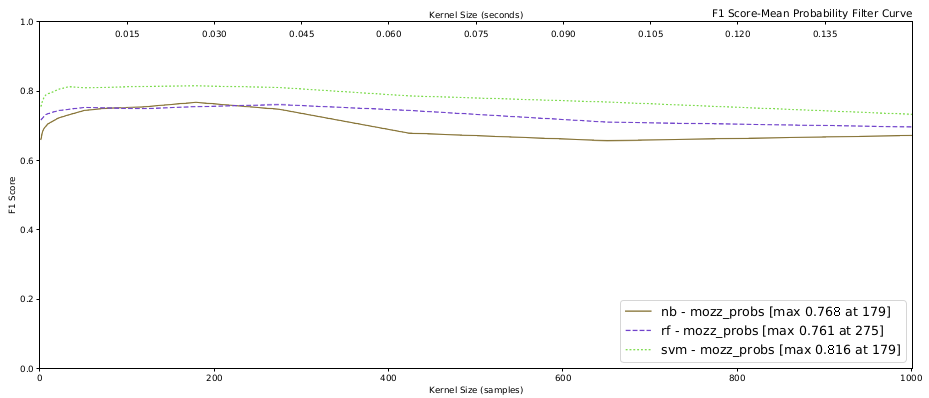
\includegraphics[width=0.9\textwidth]{meanfilt}
            \caption{F$_{1}$ scores as moving average filter kernel sizes are varied.}
            \label{fig:exp-postproc-filt}
        \end{figure}
        Kernel sizes, $K_{med}$ and $K_{mean}$, are tested over an exponential scale, decreasing from $1001$ samples (\SI{1/8}{\second}) to $3$ samples (\SI{0.375}{\milli\second}) through multiplying by powers of $0.65$. This reflects the expectation of smaller kernel sizes being more susceptible to noise and therefore producing more varied outputs. An example output graph is shown in figure \ref{fig:exp-postproc-filt}, where similar graphs have been generated for the median filter and for the metrics established previously. The best method and kernel size for filtering is chosen for each classifier. All the classifiers satisfy rejection and resolution criteria, however, only the SVM reaches the minimum true negative rate required for the lower-accuracy use case, all other metrics are unsatisfied so more work on improving accuracy is needed.

    \subsection{Rejection}
    \label{subsec:exp-postproc-rej}
        \begin{figure}[ht]
            \centering
            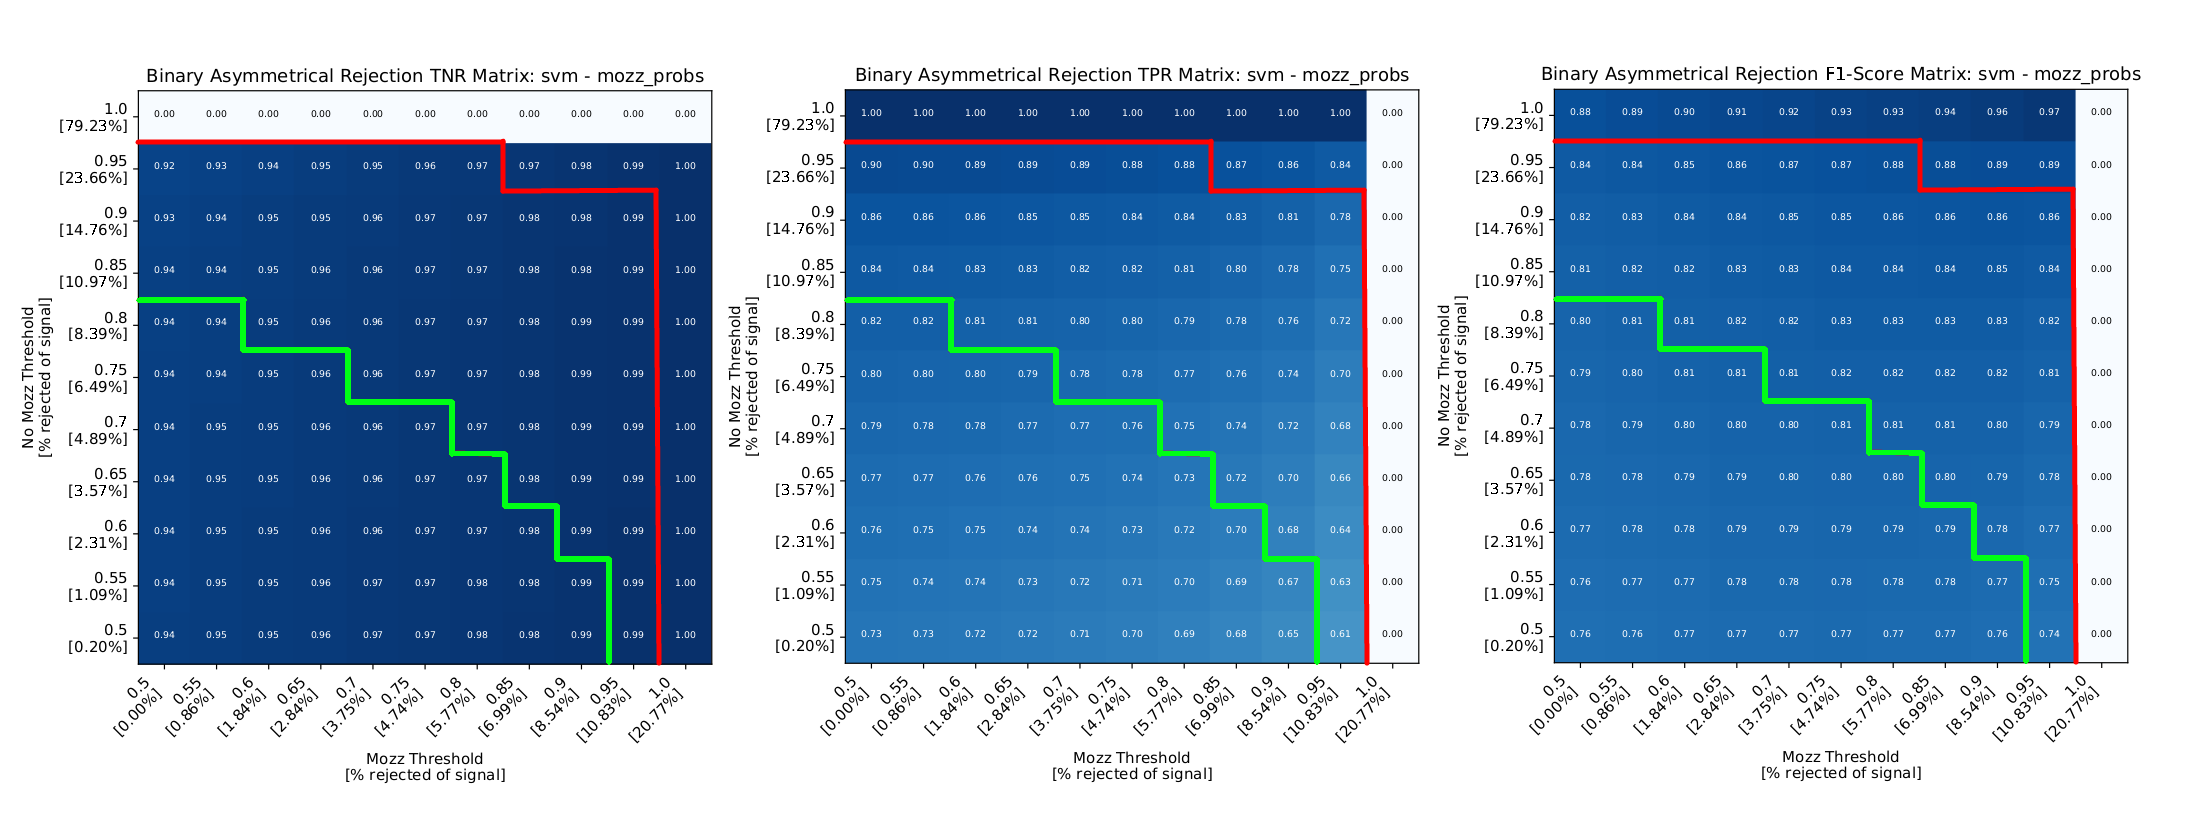
\includegraphics[width=\textwidth]{asymm_rej}
            \caption{dfgdfg}
            \label{fig:exp-postproc-asymrej}
        \end{figure}
        Accuracy can also be increased through post-processing by rejecting predictions the classifier is less certain about. Figure \ref{fig:exp-postproc-asymrej} shows three metric-rejection grids with bounds overlaid corresponding to the design specifications. 
    
    \subsection{Filtering and Rejection}